\chapter{Modell}\label{chap:model}

\section{Egyenáramú motor dinamikája}

\begin{figure}[ht]
\begin{center}
\phantomsection{}
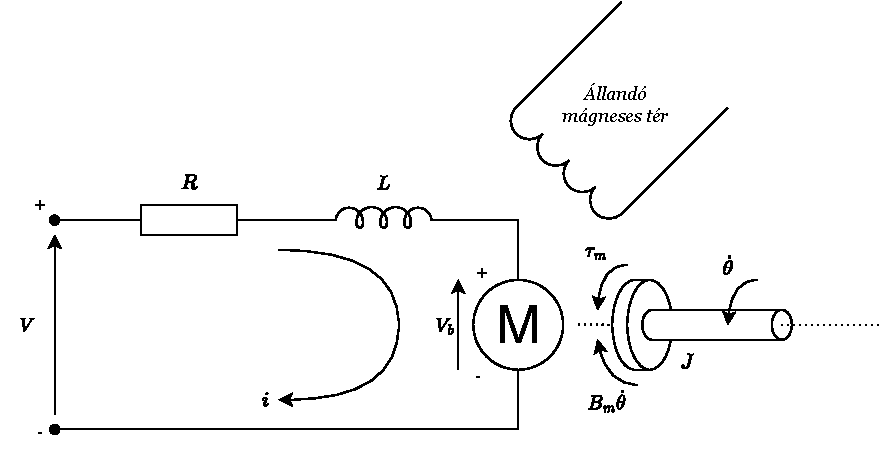
\includegraphics[width=\textwidth]{images/dc_motor_model.pdf}
\caption{Egyenáramú motor áramkör és szabadtest ábra}
\end{center}
\end{figure}

A felhasznált motor feltételezetten állandó gerjesztésű. A kifejtett nyomaték 
a Biot-Savart-törvény szerint arányos a forgorészen átfolyó árammal. A forgórészben
indukált feszültség pedig arányos a szögsebességével a Lenz-törvény alapján 
\begin{align}
    \tau_m = K_\tau i \\
    V_b = K_e \dot\theta
\end{align}
ahol $K_\tau$ a nyomatékállandó, $K_e$ a sebesség-feszültség állandó, $\tau_m$ a kifejtett 
nyomaték, $i$ a rotor árama, $V_b$ az rotorban indukált feszültség és $\dot\theta$ a rotor szögsebessége.
Az energiamegmaradás törvénye alapján a két konstans értéke megegyezik
\begin{align}
    K_m = K_\tau = K_e
\end{align}
így a következőkben $K_m$-ként jelennek meg. A forgorész áramkörére Kirchhoff I. törvénye alapján felírható
\begin{align}\label{eq:armature_circuit}
    V - Ri - L\frac{di}{dt} - K_m\dot\theta = 0
\end{align}
ahol $R$ a forgórész tekercsének ellenállása, $L$ a tekercs induktivitása, 
$K_m$ a motorállandó, $V$ a motor feszültsége, $i$ a motoráram és $\theta$ a szögelfordulás.
A forgórészt mechanikailag egy merev testként tekintve Newton II. törvénye alapján
\begin{align}\label{eq:rotor_dynamics}
    J\ddot\theta = -B_m\dot\theta + K_m i + \tau
\end{align}
ahol $J$ a forgórész tehetetlensége, $B_m$ a viszkózus csillapítási együttható, 
$K_m$ a motorállandó, $\theta$ a szögelfordulás, $i$ a motoráram és $\tau$ a forgórészre
ható külső nyomaték. Ez a két lineáris differenciálegyenlet egyértelműen leírja a 
rendszer időtartománybeli viselkedését.

A további vizsgálathoz kedvezőbb a differenciálegyenleteket állapottérmodellként felírni.
Egy állatopttérmodell általánosan
\begin{align}
    \dot{\bm x} = \bm A \bm x + \bm B \bm u \\
    y = \bm C \bm x + \bm D \bm u
\end{align} alakban írható fel. 
A két bemenet a külső nyomaték és a motorra adott feszültség. A kimenet a forgórész szöge.
A paramétereket kifejtve~\ref{eq:armature_circuit} és~\ref{eq:rotor_dynamics} alapján a modell
\begin{align}
    \frac{d}{dt}
    \begin{bmatrix}
        \theta \\
        \dot\theta \\
        i
    \end{bmatrix}
    =
    \begin{bmatrix}
        0 & 1 & 0 \\
        0 & -\frac{B_m}{J} & \frac{K_m}{J} \\
        0 & -\frac{K_m}{L} & -\frac{R}{L} \\
    \end{bmatrix}
    \begin{bmatrix}
        \theta \\
        \dot\theta \\
        i
    \end{bmatrix}
    +
    \begin{bmatrix}
        0 & 0 \\
        \frac{1}{J} & 0 \\
        0 & \frac{1}{L} \\
    \end{bmatrix}
    \begin{bmatrix}
        \tau \\
        V \\
    \end{bmatrix}
\end{align}
\begin{align}
    \theta = 
    \begin{bmatrix}
        1 & 0 & 0
    \end{bmatrix}
    \begin{bmatrix}
        \theta \\
        \dot\theta \\
        i
    \end{bmatrix}
    +
    \begin{bmatrix}
        0 & 0
    \end{bmatrix}
    \begin{bmatrix}
        \tau \\
        V \\
    \end{bmatrix}
\end{align}
alakba írható át. 

% \section{Egyenáramú motor átviteli függvénye}

% \section{Impedancia szabályozó}

% \begin{figure}[ht]
% \begin{center}
% \phantomsection{}
% 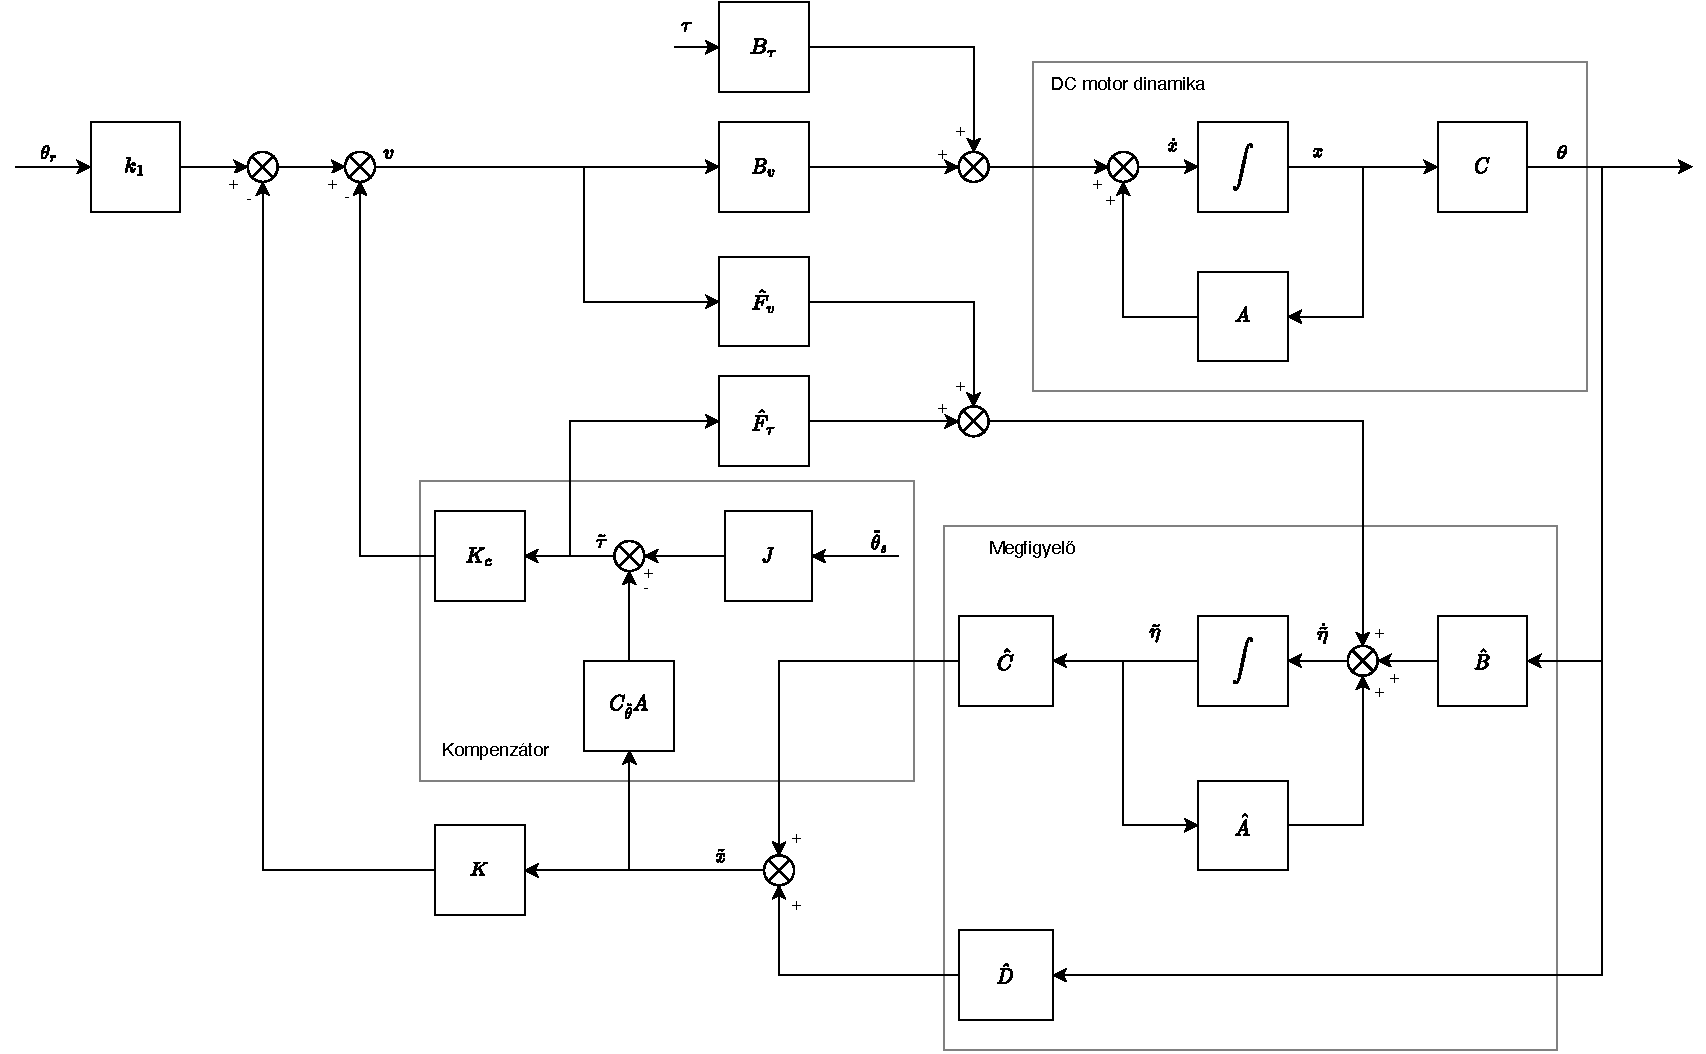
\includegraphics[width=\textwidth]{images/compensated_position_controller.pdf}
% \caption{Impedancia szabályozó szöggyorsulás méréssel}
% \end{center}
% \end{figure}
